\section{Introduction}
\subsection{Introduction to the Problem}
With the rapid development of science and technology, optimizing traffic flow has become an urgent demand of people around the world. 
Under the new conditions and prerequisites, the old rules may no longer apply. 
In order to address the problem above we conclude two sub-problems to tackle in our paper: 
\begin{itemize}
\item Analyze whether keep-right-except-to-pass rule work in new conditions including heavy traffic, more lanes, etc. 
Compare keep-right-except-to-pass rule and other alternatives and decide which is better at what need. 
Analyze its robustness. 
\item Research how will the conclusion vary providing vehicles are controled by intellegent system. 
\end{itemize}
\subsection{Background}
Attempts to produce a mathematical theory of traffic flow date back to the 1920s, when Frank Knight first produced an analysis of traffic equilibrium, which was refined into Wardrop's first and second principles of equilibrium in 1952\cite{trafficflowhistory}. 
In 1950s, CA(cellular automaton) model are raised by Von Neumann, and it called much attention in 1970s. 
S.Wolfram first implemented this model on addressing traffic flow\cite{1983RvMP...55..601W}. 
Since then quantities of CA models are proposed in the realm of traffic flow theory, such as NaSch model, FI model, BML model, etc. 
As civilization developed, old models are more and more limited. 

\subsection{Simulation Model}
We developed a new traffic flow simulation model toolkit based on HTML5. 
It's at most four rows in width and $100000$ units in length. 
With the function of collision pre-detection and fundamental diagram paiting, we can easily analyze the performance of individual strategies. 
\begin{figure}[H]
  \centering
  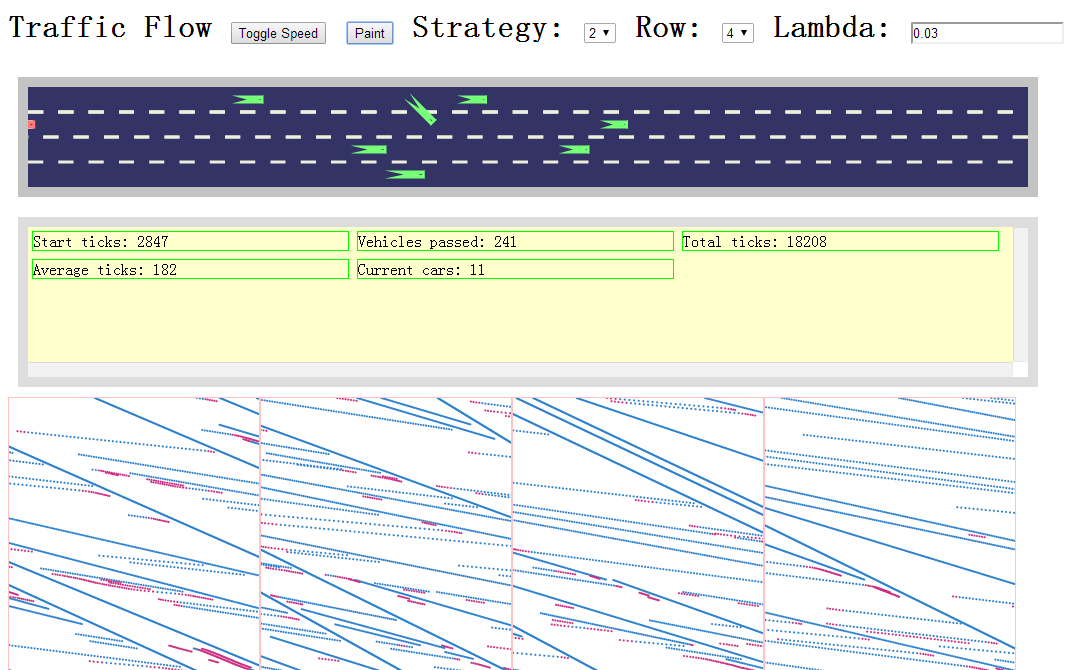
\includegraphics[width=.6\textwidth]{./img/simulationmodel.png}
  \caption{Strategy, max rows, and car amount can be changed instantly. In the fundamental diagram, blue points mean the vehicle is running at its fastest speed, red points means it's obstructed. }
  \label{fig:simulationmodel}
\end{figure}
Figure \ref{fig:simulationmodel} shows the interface simulation toolkit. 
And if we need faster calculation, we can toggle the animation and process with no delay. 
Time inside this system is based on ticks as a unit of time rather than real time, so the programme can maximize the computer capacity. 

Under this model we analyzed the formal individual strategies of vehicle drivers, estimated a trival upper bound of traffic efficiency, and tried to design an optimal self-adapting solution capable of all condition that make efficiency approach to the upper bound. 

% event loop, collision pre-detection, lane changing are expandable
\section{Nomenclature and Terminology}
\begin{table}[H]
  \center{
    \begin{tabular}{ccc}
      \toprule
      Variable & Description\\
      \midrule
      $R_m$ & Max width of the road, Counting by row from $0$. \\
      $\theta$ & Front warning ratio, impact the collision pre-detect. \\
      $a_-$ & Accelerate factor of increasing speed. \\
      $a_+$ & Accelerate factor of decreasing speed. \\
      $\lambda_p$ & Vehicles quantity factor. \\
      $V_{tot}$ & Number of total vehicles passed by. \\
      $V_{ticks}$ & Total ticks all vehicles consumed. \\
      $Cur$ & Total vehicles shown on the model \\
      $V^i$ & The vehicle with id $i$. \\
      $V^i_x$ & Distance the vehicle $V$ has traveled. \\
      $V^i_c$ & Speed of the vehivle $V$. \\
      $V^i_{c_{max}}$ & Max speed of vehicle $V$. \\
      $k$ & Density of traffic flow. \\
      $\text{tick}$ & An atom unit of time in this model. \\
      $C$ & Capacity index, \\
      \bottomrule
    \end{tabular}
  }
\end{table}
\section{Assumptions and Justification}
\subsection{Assumptions}
The argumentation in this paper is based on assumptions below. 
\begin{itemize}
\item Safety has the unconditional priority to any other goals; 
\item Roadways in this paper refer to streight equal width roadways. Vehicles travls along and across equal width lanes freely, and long term occupying more than one lane is not permitted; 
\item The amount of vehicles at each time fits Poisson distribution\cite{breiman1963}; 
\item The length and max speed of vehicles evenly distributed in specific intervals($\text{length}\in\left[150, 250\right], \text{max speed}\in\left[20, 150\right]$); 
\item As both speed and accelleration are related to the performance of the vehicle, we assumpt acelleration is linear to speed; 
\item Each vehicle will always accelerate to its max speed if there is mo concer; 
\item Traveling across lanes make a car engaging two lanes for a while, and requires no other costs; 
\item Accidents are out of account; 
\item Other enviromental condition remain stable; 
\item Tick is a atom unit of time in our model. Time is discrete and the aberration it leads to is ignored.
\end{itemize}
\subsection{Justification}
\paragraph{Capacity Index}
Let $C$ be the capacity index to describe how much is the current model capable. Define, 
\[
C=\frac{V_{ticks}}{V_{tot}}\cdot Cur. 
\]
As we see, $C$ is linear to the traffic density $k$. 
\paragraph{Collision Pre-detection}
The collisioon pre-detection can be divided into three parts: 
checking the status code, searching the horizon, and calculating warning area. 
\subparagraph{Status code}
Collision includes various situations. 
While a vehicle is crossing lanes, it engage two rows at the position. 
Thus we need a binary status code to identify the vehicle status and judge whether two vehicles are possible to collide. 

The code is just a binary expression of where the vehivle is, but it reduces much workload of writing the model. 

\subparagraph{Horizon}
We define horizon of a vehicle a set of other vehicles that it can meet within one lane changing. 
In most situation the set can describe all what a driver needs to make decisions.

\subparagraph{Warning Area}
In order to quantify the latent collision danger, and to make the threhold of collision warning clear, we define 'warning ratio' to calculate an alert area which can estimate whether two car will collide. 

We use $\theta$ to represent warning ratio. The number is calculated to avoid collision, so we have,  
\[
\theta=\frac{1}{2}\cdot\left(\frac{V_v}{a_+}\right)^2
\]
With the parameters we set, $\theta$ has the value of $24.5$. 
The warning area can be figured out with it. 

\paragraph{Event Loop}
We define 'tick' as an atom time unit. 
A tick passes means the whole model has become a new one. 
In our model, during every tick we: 
\begin{enumerate}
\item Refresh status of each vehicles; 
\item Make everyone's decision; 
\item Repaint the canvas. 
\end{enumerate}
As we tested, one tick takes about 5 miliseconds, so the fastest processing can be 200 ticks per second.  

\paragraph{Lane Changing}
We will perform the action of lane changing as follows: 
\begin{enumerate}
\item Change direction; 
\item Let the vehicle occupy the relevant two lanes;
\item Set turning status expire time and do restore the vehicle status and alter the lane.
\end{enumerate}
We tested and watched the model performance and chose $5$ as expire time to make it real.

We've successfully revealed common phenomenons of traffic flow. 
Figure \ref{fig:jam} is a good illustration of traffic jam in one lane.
\begin{figure}[H]
  \centering
  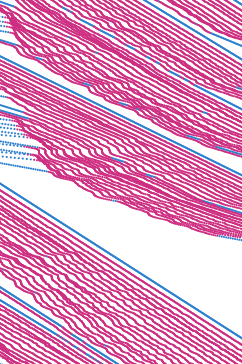
\includegraphics[width=.3\textwidth]{./img/jam.png}
  \caption{Traffic Jam}
  \label{fig:jam}
\end{figure}

\section{Analysis}
\subsection{Left or Right}
Our strategy and model doesn't acquire exact direction, but a stable one. Discussion below are based on right-hand based society. It won't matter if you swap the two directions. 

\subsection{The Keep-Right-Except-To-Pass Rule}
The keep-right-except-to-pass employ a rule that requires drivers to drive in the right-most lane unless they are passing another vehicle, in which case they move one lane to the left, pass, and return to their former travel lane. 
In old condition, bidirectional traffic requires vehicles sometime share lanes. 
So the rule of right- and left-hand traffic emerged naturely. 
Besides, there are few vehicles, and roads are narrow. And to fit the road interchange, fixing a direction is always good to unify. Figure \ref{fig:cloverleaf} shows an cloverleaf
\begin{figure}[H]
  \centering
  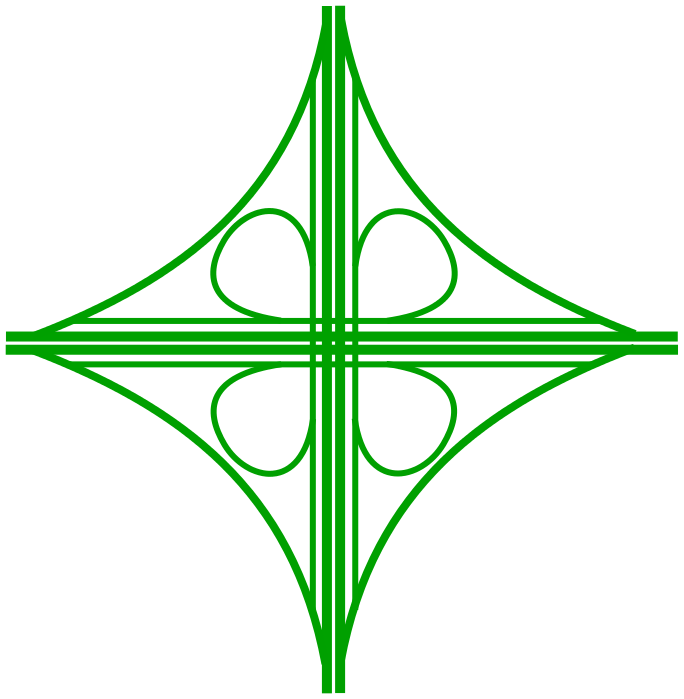
\includegraphics[width=.2\textwidth]{./img/cloverleaf.png}
  \caption{If keeping one direction is not determined, the interchanges will become a big bottleneck\cite{wikicloverleaf}. }
  \label{fig:cloverleaf}
\end{figure}
Our model Also perfectly reveal this situation. 
\begin{figure}[H]
  \centering
  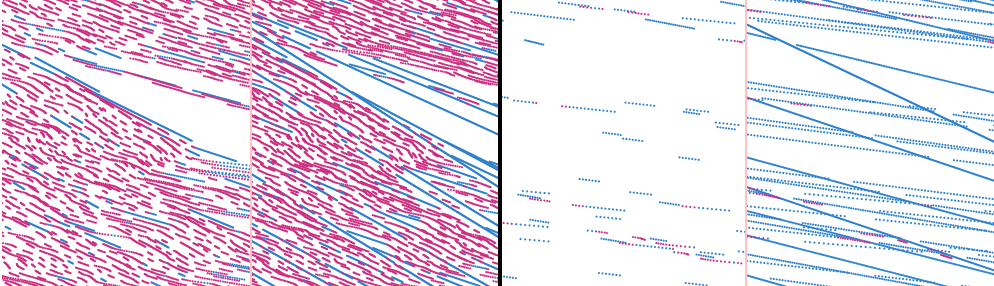
\includegraphics[width=.8\textwidth]{./img/keeprightgood.png}
  \caption{The left one shows a diagram of heavy traffic in two lanes. The right one shows that under light traffic. }
  \label{fig:keeprightgood}
\end{figure}
Figure \ref{fig:keeprightgood} shows that, on two lanes, either large amount of vehicles or few vehicles can occupy all the resourse. 
There's much few redundancy. 

However, under new condition this rule does not apply any more. 

\begin{figure}[H]
  \centering
  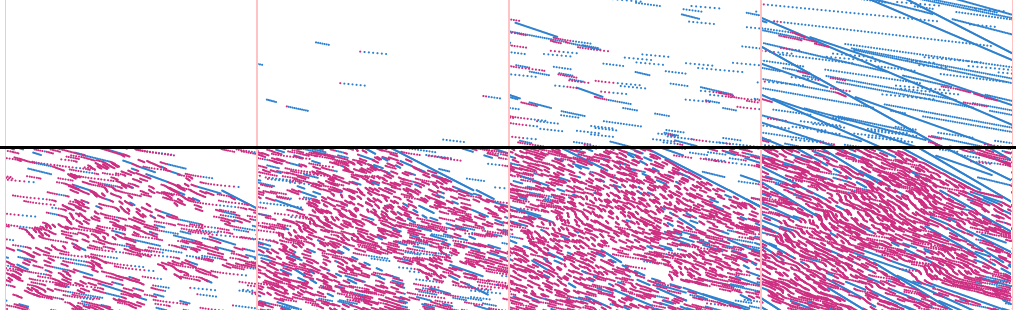
\includegraphics[width=.8\textwidth]{./img/keepright4bad.png}
  \caption{The upper one shows a diagram of light traffic in two lanes. The lower one shows that under heavy traffic. }
  \label{fig:keeprightgood}
\end{figure}
Figure \ref{fig:keeprightgood} shows that at condition of four lanes, the keep-right-except-to-pass rule has emerged its disadvantages.
At light traffic, vehicles change lanes frequently, and the left most lane is nearly vacant. 
It's a waste of time and space. 
At heavy traffic, vehicle still change lanes frequently, but remain slow all the time. 

So we can conclude that, the keep-right-except-to-pass rule does not work well now. 

\subsection{A Trival Upper Bound of Traffic Efficiency}
In order to set goals and to compare, we did an experiment of observing the trival upper bound of traffic effiency. We canceled collision pre-detection, vehicels run freely. There's no congestion. So the statistic here is an upper bound of traffic efficiency. Figure \ref{fig:graphupperbound} shows the estimated trival upper bound of traffic efficiency. 

\subsection{The Difference Between Human Judgment and Intelligent System}
When taking intelligent system into consideration, we should get to know the difference. 
Intellegent systems has rapid processing speed, sharp sensors, and fast radio communication. 
We need to refractor the model to meet new demand. 
\paragraph{Microscopic versus Marcoscopic}
Human can't see too far, and they only have two eyes. 
Though the Internet has been already universal, information cannot get comprehend as fast as it appear. 
So when intelligent system is replacing human drivers, first thing to say is Marcoscopic. 
The intelligent system can query anything it need, so the horizon will never be a limit. 

\paragraph{Individualistic versus Collectivistic}
Not only horizon is broaden, a centered dispaching system is also able to design a perfect solution that fits everyone in the situation. This can be dan if there's a leading system that direct all others. 

\paragraph{More Kinetic}
As processor runs far more faster than human, intelligent system can response very fast. 
We can analyze more deep information like higher order derivative. 
More information processed often leads to more valueable conclusion. 
And the final decision will be better. 

\section{Model \uppercase\expandafter{\romannumeral1}: Individual Strategy Under Certain Rules}
\subsection{Existent Strategy}
\paragraph{The Wait-only Strategy}
In order to compare, we add this control group. It's the safest but slowest. See figure \ref{waitless}
\begin{figure}
\begin{minipage}[t]{0.5\linewidth}
\centering
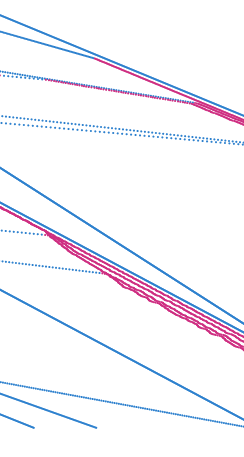
\includegraphics[width=2.2in]{/img/waitless.png}
\caption{fig1}
\label{fig:waitless}
\end{minipage}%
\begin{minipage}[t]{0.5\linewidth}
\centering
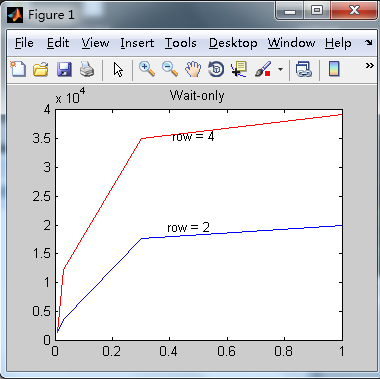
\includegraphics[width=2.2in]{./img/graphwait.png}
\caption{fig2}
\label{fig:graphwait}
\end{minipage}
\end{figure}
\paragraph{The Keep-Right-Except-To-Pass Strategy}
This strategy has just been discussed. After our test, we found this strategy only perform well in less lanes, less traffic condition, see figure \ref{graphkeepright}
\paragraph{The Speed Classifying Strategy}

\paragraph{the Dodging Strategy}
\subsection{Distinctive Strategy}

\subsection{Effeciency Analysis}

\section{Model \uppercase\expandafter{\romannumeral2}: }
... 

\section{Evaluate of the Models}
\subsection{Strengths}

\subsection{Weaknesses}

\subsection{Sensitivity and Robustness}
%��������ͨ������ʹ��ģ�͸�����ʵ��Ӧ���������ķ�����
\section{Conclusion}


\begin{thebibliography}{99}
\end{thebibliography}
%====================��¼����������==========================================
\begin{appendices}
%\renewcommand{\thesection}{\Alph{chapter}.}
\section{First appendix}
Here are simulation programmes we used in our model as follow.\\
\textbf{\textcolor[rgb]{0.98,0.00,0.00}{Input matlab source:}}
\lstinputlisting[language=Matlab]{./code/matlab1.m}
\section{Second appendix}
some more text\textcolor[rgb]{0.98,0.00,0.00}{\textbf{Input C++ source:}}
\lstinputlisting[language=C++]{./code/sudoku.cpp}
\end{appendices}

